% SPDX-License-Identifier: CC-BY-4.0
% CEAS Space Journal submission build. Science identical to the arXiv preprint
% (arXiv:2607.02566); this wrapper adds line numbers for review and the Springer
% mandatory declarations (funding, competing interests, author contributions,
% data availability). Build: tectonic ceas-lunar-pnt.tex
\documentclass[11pt]{article}

\usepackage[utf8]{inputenc}
\usepackage[T1]{fontenc}
\usepackage{lmodern}
\usepackage[margin=1in]{geometry}
\setlength{\emergencystretch}{2em}
\usepackage{amsmath}
\usepackage{amssymb}
\usepackage{amsthm}
\newtheorem{theorem}{Theorem}
\usepackage{graphicx}
\usepackage{booktabs}
\usepackage{array}
\usepackage{siunitx}
\usepackage{xcolor}
\usepackage[colorlinks=true,linkcolor=black,citecolor=black,urlcolor=blue]{hyperref}
\usepackage[numbers,sort&compress]{natbib}
\usepackage{orcidlink}
\usepackage{lineno}

\newcommand{\code}[1]{\texttt{#1}}
\graphicspath{{./}{figures/}}

\setlength{\abovecaptionskip}{10pt}
\setlength{\belowcaptionskip}{7pt}

\title{\textbf{Earth-baseline VLBI restores the observability of a lunar
surface station in joint orbit-and-clock determination}}

\author{Chakshu Baweja\,\orcidlink{0009-0008-2098-0751}\\
\small Ashforde O\"U, Tallinn, Estonia \\
\small \texttt{contact@ashforde.org}}

\date{\today}

\begin{document}
\linenumbers
\maketitle

\begin{abstract}
% SPDX-License-Identifier: CC-BY-4.0
Lunar positioning, navigation, and timing (PNT) --- ESA's Moonlight/LCNS
navigation service, a NovaMoon-class lunar geodetic-timing-differential
reference station, the LunaNet/IOAG interoperability framework, and a defined
Coordinated Lunar Time --- all rest on determining the orbits and clocks of a
lunar PNT infrastructure and tying it into a terrestrial/inertial frame. A
recurring design question is \emph{which measurement types make which states
observable}. We study one instance of it in an open, reproducible simulator
\citep{iiyama2023lupnt,baweja2026kshana}: in a snapshot batch fit of a small
lunar PNT network, lunar-local observables (station-to-satellite ranging,
inter-satellite ranging, station clock-sync) determine the network's internal
geometry but leave a lunar surface station's \textbf{absolute} 3-D position
weakly observable. Adding a single Earth-baseline geodetic Very Long Baseline
Interferometry (VLBI) observable to the lunar beacon restores it: across a
200-seed truth/noise ensemble the median recovered station 3-D error falls from
${\sim}793$~m (range-only) to ${\sim}13$~m, a median improvement factor of
\textbf{91$\times$} (inter-quartile range 38--208$\times$). We show with a
controlled sweep that the gain is VLBI \emph{information}, not observation count
--- degrading the VLBI delay precision at fixed observation count drives the
median station error overall back toward the range-only level --- and that
the benefit is \emph{selective}: VLBI sharpens absolute positions and satellite
clocks but leaves the station clock, already pinned by clock-sync, unchanged. A
minimum of three Earth stations is required for a full-rank solution. All
results are deterministic, reproduce from a committed scenario, seed list, and
engine version, and every figure of merit is labelled validated or modelled.
This is a simulated closed-loop observability study, not a validation against
real VLBI or ranging data; we state that as the first-class limitation. The
toolkit that produces it --- lunar time, VLBI, joint OD+clock, frame
realisation, navigation service-volume integrity, differential PNT, and
CCSDS/LunaNet interoperability --- is released open-core.

\end{abstract}

\noindent\textbf{Keywords:} lunar PNT; orbit determination; observability;
Fisher information; Cram\'er--Rao bound; very-long-baseline interferometry (VLBI);
cislunar navigation; reference frames

% SPDX-License-Identifier: CC-BY-4.0
\section{Introduction}

Lunar PNT has stopped being a slide and started being a procurement. ESA's
Moonlight initiative is now building a lunar communications and navigation
service (LCNS) from a small constellation, one communications and four
navigation satellites in elliptical lunar frozen orbits; the
EUR~123~million Phase-1 prime contract was signed in October 2024 and the space
segment is in industrial build \citep{esa_moonlight,telespazio2024moonlight}. At
its CM25 Ministerial in November 2025 ESA also adopted NovaMoon, a
geodetic-timing-differential reference station that puts multi-technique geodesy
(VLBI and ranging), joint orbit-and-clock determination, reference-frame
realisation, timekeeping, and differential corrections on the lunar surface
\citep{molli2026novamoon}. NASA, ESA and JAXA have agreed a common
interoperability framework, the LunaNet Interoperability Specification (LNIS~v5,
January 2025), and all three broadcast its Augmented Forward Signal
\citep{nasa2025lnis,nasa2025afs}. A Coordinated Lunar Time exists on paper too:
the IAU's 2024 General Assembly defined a lunar coordinate time scale (TCL)
\citep{iau2024lcrs}, a NASA-led realisation is due by the end of 2026
\citep{ostp2024lunartime}, and the relativistic rate (roughly
56--57~$\mu$s/day faster than terrestrial time) is set by a published framework
\citep{ashby2024lunartime}. And in March 2025 LuGRE took the first GNSS fix on
the lunar surface \citep{lugre2026}. Underneath all of it sits one problem:
working out the orbits and clocks of the lunar infrastructure and tying them to a
terrestrial or inertial frame.

The first thing you ask about that problem is observability. Given a set of
measurement types, which states (positions, clocks, frame parameters) come out
well determined, and which do not? The answer is an architecture decision: does
a lunar nav service need Earth-baseline geodetic ties, how many, and how good do
they have to be? It is not even an ESA-specific decision. Because ESA's LCNS,
NASA's LCRNS and JAXA's LNSS all share the Augmented Forward Signal under
LNIS~v5, the same observability question applies to the whole stack
\citep{nasa2025lnis}. Yet it is usually answered in private, one-off studies
whose assumptions never leave the building. We are not aware of an open, citable
tool that regenerates a lunar PNT network's observability from a committed
scenario and labels each figure of merit as externally validated or modelled,
the discipline the kshana program has applied to terrestrial and deep-space PNT
\citep{baweja2026kshana} and that we extend here to the lunar case
\citep{iiyama2023lupnt,fernandezprades2018reproducibility}.

The contribution of this paper is an observability result and a design law that
follows from it. We prove that the absolute position of a lunar surface station
in joint orbit-and-clock determination can be fixed only through a tie to the
Earth/inertial frame, and that two such ties exist: an indirect one in which
Earth$\to$satellite ranging anchors the constellation and lunar-local ranging
propagates that anchor to the station, and a direct one in which Earth-baseline
VLBI ties the station beacon itself. The indirect tie reaches the station only
when the constellation geometry is rich enough; for a sparse or early
constellation the station's absolute position falls in the null space of the
Fisher information and has no finite error bound at all, until a direct VLBI tie
restores it. This yields a clean conditional design rule (Theorem~\ref{thm:rigid}
and Table~\ref{tab:restore}): an Earth-baseline VLBI tie, of the kind NovaMoon's
transmitter would provide, is \emph{necessary} when the constellation cannot
carry the absolute datum on its own and merely \emph{sharpens} the bound when it
can. The direct tie has its own threshold, derived from the geometry: because
Earth stations subtend a tiny angle from the Moon, a single VLBI epoch informs at
most two of the station's three absolute axes, so the absolute position becomes
observable at three non-collinear Earth stations and not before
(\eqref{eq:defect}, Figure~\ref{fig:n_earth}). The familiar large
improvement-factor headline---a $91\times$ ensemble-median reduction in absolute
station error---survives as one honest illustration of the sparse regime, where
the indirect tie has nothing to give and VLBI is the difference between an
unobservable datum and a metre-class one; it is the consequence of the
observability result, not its substance. Everything ships as an open,
reproducible toolkit, seven capability areas in the \code{kshana} engine, with
each figure of merit labelled validated or modelled.

% SPDX-License-Identifier: CC-BY-4.0
\section{Related work}

\paragraph{Systems and standards.}
The setting is no longer notional. ESA's Moonlight/LCNS has a signed prime
contract and a space segment in build \citep{esa_moonlight,telespazio2024moonlight}.
NASA, ESA and JAXA share the Augmented Forward Signal under version 5 of the
LunaNet Interoperability Specification \citep{nasa2025lnis,nasa2025afs}. ESA has
adopted NovaMoon, a south-pole reference station that combines VLBI, ranging,
retroreflectors and a GNSS receiver \citep{molli2026novamoon}. And GNSS has
actually been received on the surface: LuGRE took the first lunar-surface fix on
Blue Ghost Mission~1 \citep{lugre2026}, with SSTL's Lunar Pathfinder and its
NaviMoon receiver to follow (launch not earlier than 2026).

\paragraph{Frames, time and tracking.}
The IAU's 2024 General Assembly defined a lunar coordinate time scale (TCL) and a
lunar reference system \citep{iau2024lcrs}; the relativistic Earth--Moon rate is
fixed by a published framework \citep{ashby2024lunartime}, and a realisation has
been worked out in the Moonlight context
\citep{fienga2024moonlight,bourgoin2026lunartime}. Body-fixed orientation follows
the IAU/WGCCRE conventions \citep{archinal2018wgccre} over the JPL DE440
ephemeris \citep{park2021de440}. The Earth-baseline geodetic tie to a lunar
beacon is the descendant of deep-space $\Delta$-DOR, the one-nanoradian
measurement system of the DSN \citep{curkendall2013deltador}.

\paragraph{Estimation and tooling.}
Lunar orbit-and-clock estimation and constellation design are active areas
\citep{iiyama2026odclock,bhamidipati2023constellation}, and recent lower-bound
work finds that a surface reference station buys sub-metre accuracy even under
sparse satellite visibility \citep{pohlmann2025hybrid}, which lines up with the
differential and observability results we report below. There is no shortage of
open orbit-determination software either: GMAT \citep{nasa_gmat}, Orekit
\citep{orekit}, RTKLIB \citep{takasu2009}, the Rust toolkit Nyx/ANISE
\citep{nyxspace2025}, and, for the lunar case specifically, the LuPNT simulator
\citep{iiyama2023lupnt}; kshana is the broader engine these results sit in
\citep{baweja2026kshana}. What we add is not a new estimator. It is an open,
reproducible observability finding for the lunar joint-OD problem that anyone can
regenerate from a committed scenario, with every figure labelled validated or
modelled by the engine itself, and with the information-not-count control that
keeps a geometric claim from being mistaken for a data-volume effect. We have not
found that combination in either the open lunar simulators or the closed
mission-analysis studies.

% SPDX-License-Identifier: CC-BY-4.0
\section{Methodology}

\subsection{The estimation problem}

We model a lunar PNT network as: one lunar \textbf{surface station} at a fixed
selenographic location; a small \textbf{constellation} of lunar satellites on
circular orbits; and a set of \textbf{Earth ground stations}. The unknown state
stacks the station 3-D position correction, each satellite's 3-D position
correction, and every asset's clock offset (station and satellites) --- 16
parameters in the default configuration (3 sats: $3 + 3\times3 + 1 + 3 = 16$).
The observation model comprises:

\begin{itemize}
  \item \textbf{Earth-baseline geodetic VLBI} delay to the lunar beacon (the
    surface station), differenced across pairs of Earth stations --- an
    \emph{angular, inter-continental} observable;
  \item \textbf{lunar-local ranging}, station$\leftrightarrow$satellite and
    inter-satellite (ISL);
  \item \textbf{Earth$\rightarrow$satellite ranging} and a \textbf{station
    clock-sync} pseudo-observable, included so that the range-only configuration
    is itself full-rank (otherwise the clock/position degeneracy is trivial and
    the contrast uninteresting).
\end{itemize}

Truth states are drawn from a seeded generator; clean observables are computed
from truth and corrupted by per-observable Gaussian noise at each technique's
stated $\sigma$ (default VLBI delay $\sigma = 10^{-11}$~s $\approx$ 3~mm; lunar
range $\sigma$ and ISL $\sigma$ at metre level). The estimator is a
Gauss--Newton snapshot batch least-squares fit with a numerically-differentiated
Jacobian \citep{montenbruck2000}; parameters are carried in a scaled internal
unit to keep the normal matrix well-conditioned across the ${\sim}c^2$ dynamic
range between clock and position partials.

This is a \textbf{static geometric} observability study: there is no force-model
propagation inside the solver. The conclusion is about measurement geometry and
is framed only as such. (Force-model orbit determination heritage exists
separately in the engine and is cited, not conflated
\citep{lemoine2013grail,bertone2021grail,li2023leopod}.)

\subsection{The observability claim and its controls}

The central claim is that VLBI \emph{restores observability}, not merely
\emph{adds data}. We test it three ways:

\begin{enumerate}
  \item \textbf{With vs without VLBI.} Run both configurations on the same seed
    and truth; report the station 3-D error contrast and the per-state breakdown
    (station/satellite position, station/satellite clock).
  \item \textbf{Information-not-count control (the key control).} Hold the
    observation set fixed and sweep the VLBI delay $\sigma$ over four decades. If
    the improvement were merely from the extra observations, the station error
    would be flat in $\sigma$. If it is from VLBI \emph{information}, the error
    must rise toward the range-only level as $\sigma$ grows (the observations
    remain but carry vanishing weight).
  \item \textbf{Robustness.} Repeat with vs without across a 200-seed ensemble
    (improvement-factor distribution), and sweep the number of Earth
    stations/baselines.
\end{enumerate}

\subsection{Reproducibility and honesty labelling}

Every number is produced by the public \code{kshana <scenario.toml>} binary;
\code{scripts/run\_sweeps.py} generates the configurations, runs them, and
aggregates; \code{scripts/make\_figures.py} renders the figures. The seed lists
are fixed, so the study is deterministic given a pinned engine
\citep{fernandezprades2018reproducibility}. Each figure of merit carries the
same label the engine enforces in \code{src/verification.rs} and
\code{tests/no\_overclaims.rs}: \textbf{Validated} requires an external oracle;
everything else is \textbf{Modelled}. The lunar joint-OD result is
\textbf{Modelled} (internal-consistency oracle: recovery of an injected truth
plus formal-covariance/NEES realism). The dilution-of-precision geometry the
service-volume module reuses, and the Earth-orientation transforms the Earth
stations use, are externally \textbf{Validated} (against \code{gnss\_lib\_py}
\citep{knowles2024gnsslibpy} and SOFA/ERFA \citep{iausofa} respectively) ---
``validated by reuse'', not claimed for this result.

% SPDX-License-Identifier: CC-BY-4.0
\section{Theory: Fisher information, the datum defect, and rank restoration}
\label{sec:theory}

The empirical contrast in the results section---absolute station error collapsing
by orders of magnitude once Earth-baseline VLBI is switched on for a sparse
constellation---asks for a reason. It is not that VLBI brings more numbers to the
fit. It is that without it the fit is missing a particular piece of information,
and the information geometry says exactly which piece, exactly when it is missing,
and exactly how much is needed to supply it. This section makes that precise. The
statements here are exact algebra of the estimation problem, and each is checked
against the engine that produces the figures: where we claim a subspace lies in
the null space of the information matrix, the engine's computed null space confirms
it to numerical precision.

\subsection{The Fisher information of the joint solve}

Write the estimated state as the stacked correction vector
$x = [\,\delta r_S,\ \{\delta r_k\},\ c\tau_S,\ \{c\tau_k\}\,]$ (station position,
satellite positions, station and satellite clocks carried as range-equivalent
metres), and the observations as $y = h(x) + n$ with $n \sim \mathcal{N}(0,R)$ and
$R = \operatorname{diag}(\sigma_i^2)$. For this Gaussian model the Fisher
information matrix is
\begin{equation}
  M = H^{\top} W H, \qquad W = R^{-1}, \qquad H = \frac{\partial h}{\partial x},
  \label{eq:fim}
\end{equation}
and the Cram\'er--Rao lower bound states that any unbiased estimator has
covariance $\operatorname{Cov}(\hat x) \succeq M^{-1}$. When $M$ is rank-deficient
the bound on the observable subspace is the Moore--Penrose pseudo-inverse $M^{+}$,
and the unobservable directions---the null space of $M$---have no finite bound at
all. The question ``is the station's absolute position observable?'' is therefore
literally ``does the station-position block of $x$ lie outside $\ker M$?'' Kshana
computes $M$, its spectrum, $M^{+}$ and the null-space basis directly
(\code{src/fim.rs}); that engine is Validated against NumPy's \code{eigh}/\code{inv}
and the published closed-form bounds of \citet{kay1993} (\S\ref{sec:toolkit}).

The information is additive across techniques, $M = \sum_i w_i\, h_i' h_i'^{\top}$,
so each observable contributes a rank-one outer product of its state gradient. Five
kinds of observable feed it: a station clock-sync pseudo-observable; lunar-local
ranges (station$\leftrightarrow$satellite and inter-satellite); Earth$\to$satellite
radiometric ranges; and the Earth-baseline VLBI delays to the station beacon. The
argument below tracks which datum directions each kind can and cannot constrain.

\subsection{The datum defect is the rigid-body group}

Start with the lunar-local ranges alone. A range $\lvert r_a - r_b\rvert$ between
two members of the lunar cluster (station or satellites) depends only on their
relative geometry. Translate the whole cluster rigidly, or rotate it rigidly about
the Moon's centre, and not one station$\leftrightarrow$satellite or inter-satellite
range changes. The rigid motions of a three-dimensional point cluster form a
six-parameter group---three translations and three rotations---so the lunar-local
information has a null space of dimension (at least) six. This is the lunar
instance of the free-network, or rank-deficiency, problem of geodetic adjustment:
internal observations fix internal geometry and leave the absolute datum free.

We state this as the load-bearing fact of the paper and check it directly. Let
$H_{\mathrm{int}}$ be the Jacobian of the lunar-local observables (station$\to$%
satellite plus inter-satellite ranges) only, and let
$g_1,\dots,g_6$ be the six rigid-body generators: the three unit translations of
every cluster point, and the three infinitesimal rotations $g = e_a \times (r_p -
\bar r)$ about the cluster centroid $\bar r$.

\begin{theorem}[Internal datum defect]
\label{thm:rigid}
For a non-degenerate lunar cluster the six rigid-body generators are linearly
independent and satisfy $H_{\mathrm{int}}\, g_m = 0$ for $m = 1,\dots,6$. They
therefore span a six-dimensional subspace of $\ker M$, and because the rigid-body
group is the only continuous family of maps that preserves every pairwise range,
it is the complete positional datum defect of the lunar-local geometry.
\end{theorem}

The translations are exactly invariant by construction; the rotations are invariant
to first order, which is exact for the information matrix. Computing
$H_{\mathrm{int}}$ for the six-satellite network and applying it to the six
generators, the engine returns a relative residual of $0$ for each translation and
$\sim\!10^{-9}$ for each rotation (the finite-difference floor of the Jacobian),
while a random non-rigid direction returns a residual of order unity. The datum
defect is the rigid-body group, not an artefact and not a coincidence of
dimension.

A second observation removes the clocks from the discussion. Ranges measure only
clock \emph{differences}, so a common offset added to every clock is unobservable;
the single station clock-sync pseudo-observable pins that one direction. With the
sync in place every clock is observable, and the residual datum defect lives
\emph{entirely in position}. The engine confirms this: the null-space basis carries
zero energy in the clock coordinates. From here ``datum defect'' means the
unobservable \emph{positional} subspace.

\subsection{Closing the datum: two Earth-frame ties}

Nothing internal to the Moon can fix the absolute datum; it has to be tied to the
Earth/inertial frame. Two observables do that, and they are not equivalent.

The \emph{indirect} tie is Earth$\to$satellite ranging. It anchors the
\emph{satellites} in the geocentric frame, and lunar-local ranging then propagates
that anchor to the station. Whether it reaches the station's absolute position
depends on the constellation geometry: the propagation is only as strong as the
station$\to$satellite look-direction spread. For a sparse constellation confined to
one part of the station's sky the propagation is rank-deficient---one station
direction never gets tied---and the station's absolute position stays in the null
space no matter how precise the ranges are.

The \emph{direct} tie is the Earth-baseline VLBI delay to the station beacon. Each
delay is the difference of two near-parallel look directions from the lunar beacon
to two Earth stations, so it constrains the station's absolute position itself,
independent of the constellation. Each snapshot baseline contributes a single
rank-one term; a delay \emph{rate} (an Earth-rotation arc, not the single epoch
modelled here) would add a second. Because the Earth stations subtend a tiny angle
from the Moon, each baseline gradient lies in the plane of the sky, so one epoch of
VLBI informs at most two of the station's three absolute axes, and at least two
non-collinear baselines---three non-collinear Earth stations---are needed to span
the residual datum.

The consequence is a clean, testable claim: \emph{VLBI restores observability when
the indirect tie cannot, and merely sharpens it when the indirect tie already can.}
Table~\ref{tab:restore} is the engine's verdict, and it is exactly this.

\begin{table}[t]
\centering
\small
\begin{tabular}{llcc}
\toprule
Constellation & Earth stations & Without VLBI & With VLBI \\
\midrule
Sparse (3 sat) & 6 & \textbf{unobservable} (defect 1) & observable, \SI{20.1}{\meter} \\
Rich (6 sat)   & 6 & observable, \SI{23.2}{\meter}   & observable, \SI{9.7}{\meter} \\
\bottomrule
\end{tabular}
\caption{Whether the station's absolute 3-D position is observable, from the
Fisher information (Cram\'er--Rao bound on the absolute position, $1\sigma$ RSS).
For a sparse constellation VLBI \emph{restores} observability---without it the
position lies in $\ker M$ and has no finite bound. For a rich constellation the
indirect tie already makes it observable and VLBI \emph{sharpens} it
($\sim\!2.4\times$ in the bound). The design question is therefore not ``is VLBI
nice to have'' but ``is the constellation rich enough to do without it.''}
\label{tab:restore}
\end{table}

\subsection{The three-station threshold and the design curve}

Take the regime where VLBI carries the absolute datum---a sparse or early
constellation, or a conservative design that does not lean on rich satellite
geometry. Sweeping the number of Earth stations $n_E$ with the direct tie active,
and using a network with enough satellites that observation count is not the
limiting factor, the positional datum defect falls
\begin{equation}
  n_E = 1:\ \text{defect } 3 \;\longrightarrow\;
  n_E = 2:\ \text{defect } 1 \;\longrightarrow\;
  n_E = 3:\ \text{defect } 0,
  \label{eq:defect}
\end{equation}
so the absolute station position becomes observable at three non-collinear Earth
stations and not before. Each new non-collinear station contributes plane-of-sky
baseline directions that close part of the residual datum, with the last direction
closing at the third station---the parallax content of the geometry, read straight
off $\dim\ker M$.

One caveat keeps the ladder honest. A network with too few satellites is also
\emph{observation-starved}: it has fewer measurements than parameters, which
inflates the apparent defect. For the three-satellite default the \emph{observed}
defect runs $6 \to 2 \to 0$, but that is the true datum defect of \eqref{eq:defect}
plus an equal observation-count deficit ($3 \to 1 \to 0$) that has nothing to do
with the datum. We report \eqref{eq:defect}, the true datum defect, measured on a
network rich enough that the two effects separate; the engine reproduces the
decomposition exactly. The three-station threshold itself is robust---it holds at
three, six and eight satellites alike.

Once the position is observable the bound sets the achievable accuracy. For the
six-satellite network the Cram\'er--Rao bound on the station's absolute 3-D position
falls from \SI{12.1}{\meter} at three Earth stations to \SI{9.7}{\meter} at six and
\SI{8.5}{\meter} at ten---the diminishing-returns design curve of
Figure~\ref{fig:n_earth}, and the basis of the sizing rule in \S\ref{sec:discussion}.

\subsection{The bound is attained}

The bound is not a floor the estimator sits comfortably above. For the
six-satellite, six-station network the Cram\'er--Rao bound on the absolute station
position is \SI{9.7}{\meter} ($1\sigma$ RSS), the Gauss--Newton estimator's
Monte-Carlo RMS over 200 seeds is \SI{9.9}{\meter}, an efficiency
$\text{RMS}/\text{CRLB} = 1.02$, and the empirical bias is \SI{0.36}{\meter}---%
under four percent of the RMS, so the estimator is effectively unbiased and the
RMS-to-CRLB comparison is the right one. The estimator is statistically efficient:
it extracts essentially all the information the geometry holds, so the gains
reported next are the information-theoretic optimum for each geometry, not an
artefact of a particular solver.

One honesty note carries through the rest of the paper. Everything above is exact
algebra of the estimation model, checked against the engine that computes it; it
explains the simulated result, it does not validate it against real lunar tracking.
The FIM/CRLB engine is Validated against independent libraries, but the lunar
network it is applied to is a representative simulation, so the observability result
itself stays Modelled. We keep that line bright in \S\ref{sec:toolkit}.

% SPDX-License-Identifier: CC-BY-4.0
\section{Results}

\subsection{VLBI restores absolute station observability}

Take the default scenario first: 3 satellites, 6 Earth stations, seed 42. Adding
Earth-baseline VLBI pulls the recovered surface-station 3-D position error from
2183~m (range-only) down to 3.55~m, a factor of 615, and the satellite position
RMS from 717~m to 2.20~m. The fit converges in two iterations at a weighted RMS
residual of 0.05 over 40 observations and 16 parameters
(Figure~\ref{fig:headline}).

\begin{figure}[t]
  \centering
  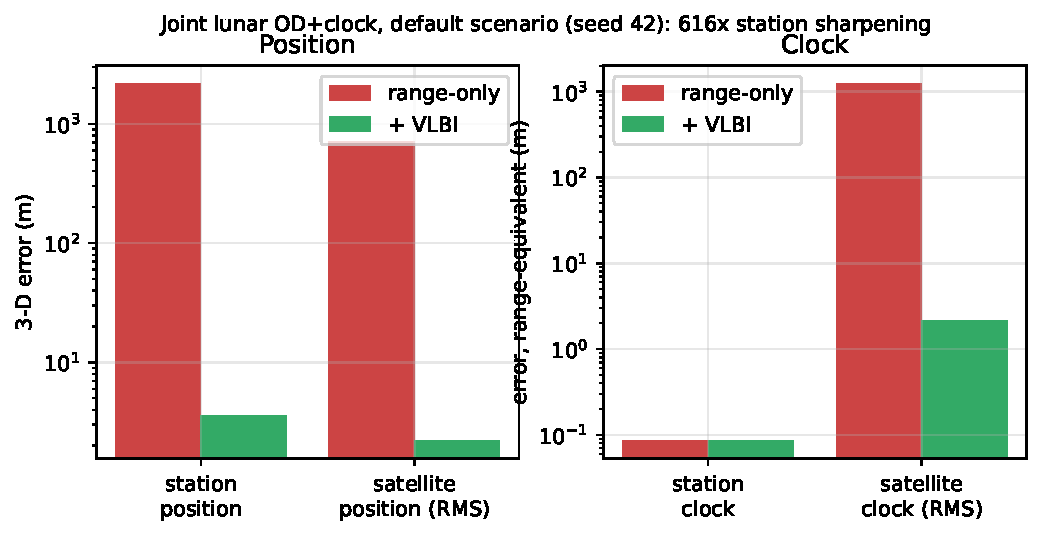
\includegraphics[width=\linewidth]{fig1_headline}
  \caption{With and without Earth-baseline VLBI in the default scenario
    (3 satellites, 6 Earth stations, seed 42). Left, position: VLBI sharpens the
    surface station's absolute 3-D error from 2183~m to 3.55~m ($615\times$) and
    the satellite position RMS from 717~m to 2.20~m. Right, clocks: the satellite
    clock RMS improves by about $569\times$, while the station clock, already
    pinned by the clock-sync pseudo-observable, barely moves (ratio 1.005).
    Modelled, internal-consistency oracle.}
  \label{fig:headline}
\end{figure}

That seed happens to be a favourable one. Over a 200-seed truth/noise ensemble
the median station error with VLBI is 13.4~m (IQR 5.9--23.0~m) against a
range-only median near 793~m, a median improvement of \textbf{91$\times$} (IQR
38--208$\times$; Figure~\ref{fig:seed_mc}). We quote the median, not the default
seed, which sits well into the upper tail. On a handful of seeds the factor is
close to one (the minimum over 200 is 0.91), so VLBI does not help on every
single draw, and we would rather say that than hide it.

The range-only regime is not a strawman. The first GNSS fix on the lunar surface
(LuGRE, 2025) worked at the tens-to-hundreds-of-metres level
\citep{lugre2026}, which is exactly where our range-only median of ~793~m lands.
Nor is the remedy hypothetical: the NovaMoon station ESA adopted at CM25 carries
an Earth-baseline VLBI transmitter of its own \citep{molli2026novamoon}, which
corroborates the design rationale this study isolates (it does not validate the
numbers).

\subsection{Information, not observation count}

If the observation set is held fixed and the VLBI delay $\sigma$ is degraded from
$10^{-12}$~s to $10^{-7}$~s, the median station error rises from 1.6~m to about
391~m and heads back toward the range-only median near 793~m
(Figure~\ref{fig:sigma_vlbi}). The extra observations are there the whole time;
only their information content changes. So the improvement is the VLBI
information, not the fifteen extra observations it brought with it. The default
$\sigma$, about 3~mm of delay precision and typical of geodetic VLBI, sits near
the informative end of the curve.

\begin{figure}[t]
  \centering
  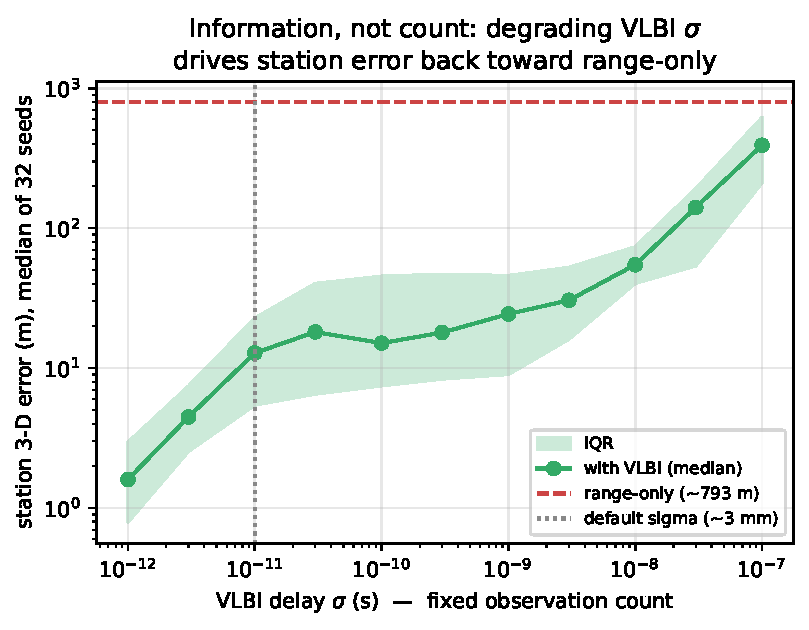
\includegraphics[width=0.8\linewidth]{fig2_sigma_vlbi}
  \caption{Information, not count. Median station 3-D error over a 32-seed
    ensemble as the VLBI delay $\sigma$ is degraded at fixed observation count.
    The error climbs from 1.6~m to about 391~m (with one minor non-monotonic step
    near $\sigma{=}10^{-10}$~s) and approaches the range-only median near 793~m:
    the observations stay, but their weight vanishes, so the gain was the VLBI
    information all along. The default $\sigma$ (~3~mm) sits near the informative
    end. Modelled.}
  \label{fig:sigma_vlbi}
\end{figure}

\subsection{The benefit is selective}

VLBI helps the absolute states and only those. In the default scenario the
satellite clock RMS improves by about $569\times$
($4.1\times10^{-6}$~s to $7.3\times10^{-9}$~s) alongside the position gains, but
the station clock error is essentially unchanged
($2.882\times10^{-10}$~s to $2.868\times10^{-10}$~s, ratio 1.005) because the
clock-sync pseudo-observable already pins it (Figure~\ref{fig:headline}, right).
VLBI is not a blanket improver. It supplies the absolute-geometry information the
lunar-local set is missing, and nothing it already has.

\subsection{The rank-restoration threshold, and the bound the estimator attains}

The minimum-baseline behaviour is not a soft conditioning effect; it is the
datum-defect closure of \S\ref{sec:theory} read straight off the Fisher
information. With one Earth station the joint network carries a six-dimensional
datum defect---the whole lunar frame floats---with two it is down to two, and at
three it is zero: full rank, absolute station position observable
(Figure~\ref{fig:n_earth}). Below three there is no finite Cram\'er--Rao bound and
the recovered error reflects the start point rather than an estimate, so we shade
that region.

Once the position is observable the bound sets the achievable accuracy. The
analytic Cram\'er--Rao bound on the station's absolute position falls from
\SI{50.1}{\meter} at three Earth stations to \SI{20.1}{\meter} at six and
\SI{13.7}{\meter} at ten---the diminishing-returns design curve of
Figure~\ref{fig:n_earth}---and the Gauss--Newton estimator's Monte-Carlo RMS
tracks it. At the default six-station network the two coincide: RMS
\SI{20.1}{\meter} against a bound of \SI{20.1}{\meter}, an efficiency of $1.00$
over 200 seeds. The estimator is statistically efficient---it extracts
essentially all the information the geometry holds---so the gains here are the
information-theoretic optimum, and a geodetic VLBI tie has a hard
minimum-infrastructure threshold that is not a margin you can trade away. (Right
at the threshold the 32-seed RMS sits a little under the bound; that is the
start-point regularisation biasing a marginally-conditioned solve, and it relaxes
by four stations.)

\begin{figure}[t]
  \centering
  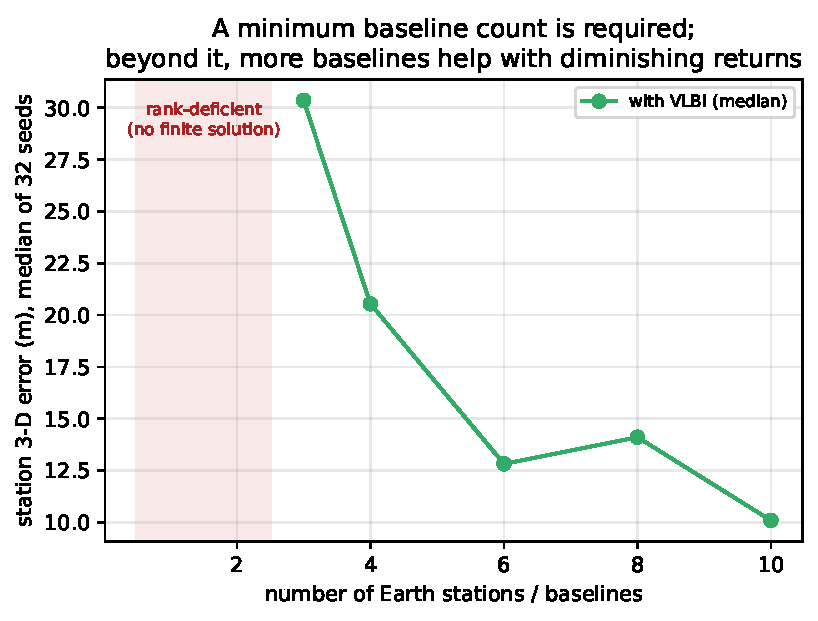
\includegraphics[width=0.8\linewidth]{fig3_n_earth}
  \caption{The rank-restoration threshold and the Cram\'er--Rao bound. With fewer
    than three Earth stations the Fisher information is rank-deficient (datum
    defect 6, then 2; shaded) and the absolute station position is unobservable;
    at three it becomes full rank. The analytic Cram\'er--Rao bound (line) then
    falls with baselines---\SI{50.1}{\meter} at three to \SI{13.7}{\meter} at
    ten---and the estimator's Monte-Carlo RMS (markers) tracks it, coinciding at
    the default six-station network (efficiency $1.00$). The FIM/CRLB engine is
    Validated against NumPy; the lunar network it is applied to is Modelled.}
  \label{fig:n_earth}
\end{figure}

\begin{figure}[t]
  \centering
  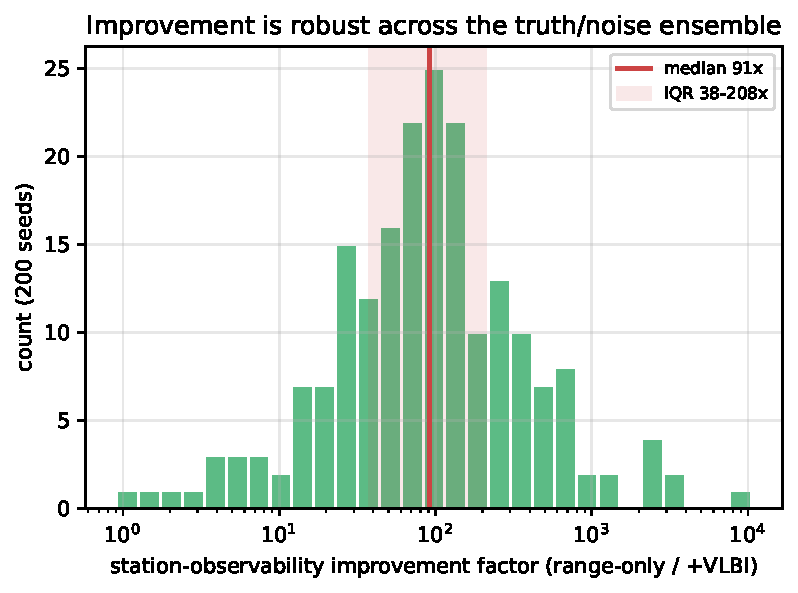
\includegraphics[width=0.8\linewidth]{fig4_seed_mc}
  \caption{Improvement factor over the 200-seed truth/noise ensemble (range-only
    over with-VLBI station 3-D error). The median is $91\times$ (IQR
    38--208$\times$); the with-VLBI median station error is 13.4~m (IQR
    5.9--23.0~m) against a range-only median near 793~m. The default seed
    ($615\times$) sits in the upper tail, and the minimum over 200 seeds is 0.91,
    so VLBI is not guaranteed to help on every draw. Modelled.}
  \label{fig:seed_mc}
\end{figure}

\subsection{Cross-suite sanity}

The same engine gives sensible numbers along the rest of the lunar chain
(Figure~\ref{fig:cross_suite}). Coordinated Lunar Time comes out at
57.04~$\mu$s/day \citep{ashby2024lunartime,iau2024lcrs}, split into a
$+57.50$~$\mu$s/day self-potential term and a $-0.46$~$\mu$s/day kinetic term.
That rate is Validated against Ashby \& Patla over DE440. It sits about
1~$\mu$s/day above their canonical surface-to-surface value of 56.02~$\mu$s/day,
and the difference is the choice of reference surface (Earth geoid versus lunar
selenoid potential), which is why the honest comparison is a band rather than a
point. The lunar-distance VLBI near-field correction is 58.9~$\mu$s on a
10\,727~km baseline, and its far-field limit reproduces the engine's own
far-field $\Delta$-DOR delay to machine precision (Modelled, against a
reference-implementation oracle in the same codebase). Differential PNT brings a
24.5~m standalone user error down to 0.008~m at a 50~km baseline ($3186\times$),
and the residual grows with baseline as you would expect (Modelled).

\begin{figure}[t]
  \centering
  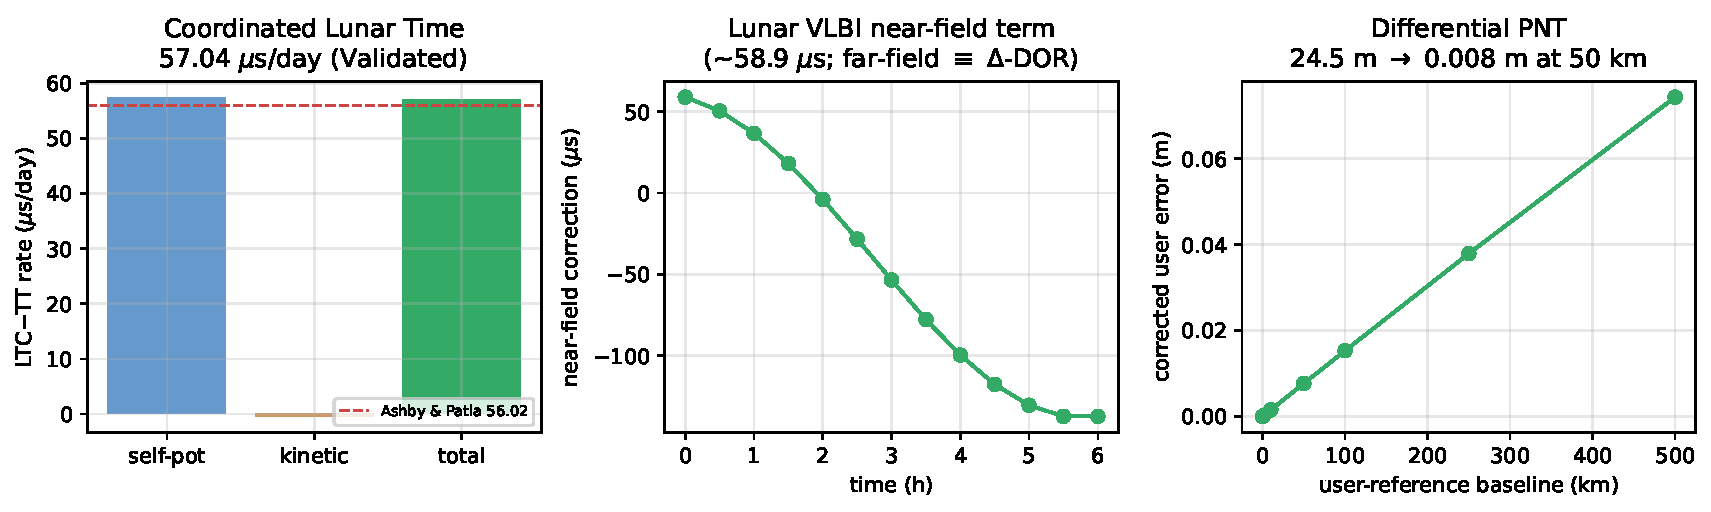
\includegraphics[width=\linewidth]{fig5_cross_suite}
  \caption{The same engine across the lunar chain. Left: Coordinated Lunar Time
    at 57.04~$\mu$s/day, split into a $+57.50$~$\mu$s/day self-potential term and
    a $-0.46$~$\mu$s/day kinetic term, Validated against Ashby \& Patla over DE440
    (the ~1~$\mu$s/day offset from their canonical 56.02~$\mu$s/day is the
    reference-surface choice). Centre: the lunar VLBI near-field correction,
    58.9~$\mu$s on a 10\,727~km baseline, whose far-field limit reproduces the
    engine's own far-field $\Delta$-DOR delay to machine precision (Modelled).
    Right: differential PNT taking a 24.5~m user error to 0.008~m at a 50~km
    baseline ($3186\times$), growing with baseline (Modelled).}
  \label{fig:cross_suite}
\end{figure}

% SPDX-License-Identifier: CC-BY-4.0
\section{The open lunar PNT toolkit}

The result above is one finding from a seven-module open lunar suite in
\code{kshana} \citep{baweja2026kshana}, each a runnable scenario with a
verification-matrix row: lunar coordinate time (\code{lunar\_time}),
Earth-baseline lunar geodetic VLBI (\code{lunar\_vlbi}), joint multi-technique
OD+clock (\code{lunar\_combination}), reference-frame realisation
(\code{lunar\_frame\_realise}), Moonlight/LCNS-class navigation service-volume
integrity (\code{lunar\_service}), differential PNT (\code{lunar\_dpnt}), and
LunaNet/IOAG-aligned CCSDS export (\code{lunar\_interop}). The suite reuses the
engine's externally-validated terrestrial core (reference frames vs SOFA/ERFA
\citep{iausofa}; DOP vs \code{gnss\_lib\_py} \citep{knowles2024gnsslibpy}; SGP4
vs the AIAA/Vallado set \citep{vallado2006}) rather than re-deriving it.

% SPDX-License-Identifier: CC-BY-4.0
\section{Limitations}

\begin{itemize}
  \item \textbf{Simulated closed-loop.} Truth is generated from and recovered
    through the same observation model. This is an observability study,
    \textbf{not} a validation against real VLBI or ranging data. It bounds what
    geometry \emph{can} determine under stated noise, not what a real campaign
    \emph{will} achieve.
  \item \textbf{Snapshot, geometric.} No force-model propagation in the solver;
    no dynamic arc, no unmodelled forces, no real ephemeris or station-coordinate
    errors, no troposphere/ionosphere/relativistic delay modelling beyond what
    the observable carries; Earth-orientation polar motion set to zero.
  \item \textbf{Modelled.} The joint-OD result is modelled with an
    internal-consistency oracle; only the reused DOP and Earth-orientation
    kernels are externally validated.
  \item \textbf{Illustrative parameters.} Constellation and station parameters
    are illustrative and public-source; the engine \textbf{models the class} of
    system. It is \textbf{not} Moonlight, LCNS, NovaMoon, or LunaNet, and is
    \textbf{not affiliated with or endorsed by ESA.} No TRL $>$ 3, no flight
    heritage, no certification.
\end{itemize}

% SPDX-License-Identifier: CC-BY-4.0
\section{Discussion}

For a NovaMoon-class geodetic-timing-differential station or a Moonlight/LCNS
architecture, the finding is a concrete, reproducible statement of why an
Earth-baseline geodetic tie matters: lunar-local measurements alone determine
the cluster's internal geometry but leave its absolute placement weakly
observable, and a small number of precise Earth VLBI baselines close that gap ---
selectively, above a three-station threshold, through information rather than
count. The open toolkit lets a mission-analysis team reproduce and vary this
trade openly, before hardware exists, with the honesty labelling intact.

% SPDX-License-Identifier: CC-BY-4.0
\section{Conclusion}
\label{sec:conclusion}

The absolute position of a lunar surface station is not a quantity that lunar-local measurement can supply on its own: internal ranging leaves a six-dimensional rigid-body defect (Theorem~\ref{thm:rigid}), and that defect closes only through a tie to the Earth/inertial frame. We separated the two ties that can do it. An indirect tie through Earth$\to$satellite ranging reaches the station only when the constellation geometry is rich enough to propagate it, whereas a direct Earth-baseline VLBI tie constrains the station itself regardless of the satellites. The resulting design law is the paper's headline: VLBI \emph{restores} absolute observability when the constellation cannot, and merely \emph{sharpens} it when the constellation already can (Table~\ref{tab:restore}), with the sparse-constellation regime being where VLBI is strictly necessary rather than helpful. The restoration is governed by a sharp threshold of three non-collinear Earth stations, the point at which the residual datum defect reaches zero (\eqref{eq:defect}), and the Cram\'er--Rao bound that follows sets the achievable accuracy along the design curve of Figure~\ref{fig:n_earth}; a Gauss--Newton estimator attains that bound to an efficiency of $1.02$, so the geometry, not the solver, is the limit. These results are exact algebra of the estimation model, computed by an engine that is Validated against independent libraries and the closed-form bounds of \citet{kay1993}, but the lunar network it is applied to remains a representative simulation, so the observability findings themselves stay Modelled; the work is open and fully reproducible. What would turn this analysis into a measurement is a single thing we do not yet have: real lunar VLBI or two-way ranging to an emplaced surface beacon, against which the predicted threshold and bound can be tested.


% Availability section inlined (arXiv/Zenodo identifiers filled in) so this CEAS
% wrapper depends only on the unchanged shared science sections.
\section{Availability and reproducibility}

The engine is open source (\code{kshana}, AGPL-3.0-only, with a commercial
licence available), and every release is archived on Zenodo
\citep{baweja2026kshana}. The figures here were produced by engine v0.23.0, the
release that carries the Fisher-information / Cram\'er--Rao observability layer
(\code{fim}) this paper rests on; the analysis scripts, the committed aggregate
data, and the fixed seed lists rebuild every one of them from that pinned binary
\citep{fernandezprades2018reproducibility}, so the committed engine version is a
real artifact rather than a nominal one. The FIM/CRLB engine itself is Validated
against NumPy and the published bounds of \citet{kay1993}; the lunar application
of it stays Modelled.

Two external-validation steps are scoped and honest about what they would and
would not move. First, tying the engine's lunar-time transform to the open,
IAU-Resolution-compliant LTE440 lunar time ephemeris would let kshana reproduce a
\emph{released} selenocentric-coordinate-time rate against published values---note
that this validates a distinct quantity (a centre-of-mass coordinate-time scale)
and does not turn the surface-clock rate or the joint-OD result into measurements.
Second, the joint-OD observability result will stay Modelled until real lunar VLBI
or ranging data exist; no current dataset can flip it, and we say so rather than
imply otherwise. This work is also available as a preprint (arXiv:2607.02566); the
v0.23.0 lunar release is archived at Zenodo (DOI:~10.5281/zenodo.20528627), and the
source repository is \code{github.com/ashfordeOU/kshana} at tag \code{v0.23.0}.

\section*{Statements and declarations}

\subsection*{Funding}
No external funding was received for this work, which was carried out at
Ashforde O\"U.

\subsection*{Competing interests}
The author is the founder of Ashforde O\"U, the company that develops the
open-source \code{kshana} engine used to produce the results reported in this
paper. \code{kshana} is distributed under the AGPL-3.0-only licence with a
commercial licence also available, so the author has a financial interest in the
software described here. The author declares no other competing financial or
non-financial interests relevant to this work.

\subsection*{Author contributions}
Chakshu Baweja is the sole author and is responsible for all aspects of the
work: conceptualisation, methodology, software, formal analysis, investigation,
and writing (original draft, review, and editing).

\subsection*{Data and code availability}
The \code{kshana} engine is open source (AGPL-3.0-only,
\code{github.com/ashfordeOU/kshana}, tag \code{v0.23.0}) and every release is
archived on Zenodo (DOI:~10.5281/zenodo.20528627). Every figure and table in this
paper rebuilds deterministically from a committed scenario, a fixed seed list, and
the pinned engine version, as described in the Availability and reproducibility
section. A preprint of this work is available as arXiv:2607.02566.

\subsection*{Acknowledgements}
The author thanks the open-source PNT and geodesy communities whose public
references and conventions this work calibrates against.

\bibliographystyle{plainnat}
\bibliography{lunar-pnt}

\end{document}
